\documentclass{acm_proc_article-sp}

\newcommand{\claim}[1]{#1}

\begin{document}

\title{Identifying change patterns in software history}

%
% You need the command \numberofauthors to handle the 'placement
% and alignment' of the authors beneath the title.
%
% For aesthetic reasons, we recommend 'three authors at a time'
% i.e. three 'name/affiliation blocks' be placed beneath the title.
%
% NOTE: You are NOT restricted in how many 'rows' of
% "name/affiliations" may appear. We just ask that you restrict
% the number of 'columns' to three.
%
% Because of the available 'opening page real-estate'
% we ask you to refrain from putting more than six authors
% (two rows with three columns) beneath the article title.
% More than six makes the first-page appear very cluttered indeed.
%
% Use the \alignauthor commands to handle the names
% and affiliations for an 'aesthetic maximum' of six authors.
% Add names, affiliations, addresses for
% the seventh etc. author(s) as the argument for the
% \additionalauthors command.
% These 'additional authors' will be output/set for you
% without further effort on your part as the last section in
% the body of your article BEFORE References or any Appendices.

\numberofauthors{2} %  in this sample file, there are a *total*
% of EIGHT authors. SIX appear on the 'first-page' (for formatting
% reasons) and the remaining two appear in the \additionalauthors section.
%
\author{
% You can go ahead and credit any number of authors here,
% e.g. one 'row of three' or two rows (consisting of one row of three
% and a second row of one, two or three).
%
% The command \alignauthor (no curly braces needed) should
% precede each author name, affiliation/snail-mail address and
% e-mail address. Additionally, tag each line of
% affiliation/address with \affaddr, and tag the
% e-mail address with \email.
%
% 1st. author
\alignauthor
Jason Dagit\\
       \affaddr{Galois, Inc}\\
       \affaddr{Portland, OR}\\
       \email{dagit@galois.com}
% 2nd. author
\alignauthor
Matthew Sottile\\
       \affaddr{Galois, Inc}\\
       \affaddr{Portland, OR}\\
       \email{mjsottile@gmail.com}
}
\date{4 July 2013}
% Just remember to make sure that the TOTAL number of authors
% is the number that will appear on the first page PLUS the
% number that will appear in the \additionalauthors section.

\maketitle
\begin{abstract}

Traditional algorithms for detecting differences in source code focus on
differences between lines.  As such, little can be learned about abstract
changes that occur over time within a project.  Structural differencing on the
program parse tree reveals changes at the syntactic level within code, which
allows us to further process the differences to understand their meaning. We
propose that clustering of changes by some metric of similarity, followed by
pattern extraction via antiunification will allow us to identify patterns of
change  within a software project from the sequence of changes contained
within a Version Control System (VCS). Tree similarity metrics such as a tree
edit distance can be used to cluster changes in order to identify groupings
that may represent a single class of change (e.g., adding a
parameter to a function call). By applying antiunification within each cluster
we are able to generalize from families of concrete changes to patterns of
structural change. Studying patterns of change at the structural level,
instead of line-by-line, allows us to gain insight into the evolution of
software.

\end{abstract}

% TODO: edit categories
% A category with the (minimum) three required fields
\category{H.4}{Information Systems Applications}{Miscellaneous}
%A category including the fourth, optional field follows...
\category{D.2.8}{Software Engineering}{Metrics}[complexity measures, performance measures]

%\terms{Theory} % TODO: changeme

\keywords{version control, structural differencing, anti-unification, software evolution}

\section{Introduction}
%% 1. Describe the problem

Version control systems (VCS's) track the evolution of software over time in the form
of a sequence of changes to the plain text representation of the code.
We would like to be able to characterize the changes to files in a software
project according to the type of change that they represent.  The ability to
map these changes to the syntax of the language, instead of its raw text
representation, will allow them to be understood in terms of the language
constructs themselves.  Doing so will allow us to identify patterns of
changes at the abstract syntax level to support insight at a deeper level
than achievable by examining raw text differences.  For example, in
an operating system kernel, a set of drivers may need to be updated to use a
new mutual exclusion mechanism. In this example, blocks of code that access
specific resources need to be updated to take a semaphore before proceeding.

Finding common patterns for the changes to a source file gives us the ability
to understand, at a higher level, what sorts of revisions are happening. If we
already know to look for changes to semaphore handling we may think to use a
textual search tool, such as {\tt grep}, to search the source code for
functions related to semaphores. Instead, suppose we have the challenge that we
are not familiar with the source code and we would like to understand at a
structural level what types of changes were needed to add support for the new
semaphores.

Furthermore, 

\claim{Finding edit patterns in source code is a hard problem.}

%% 2. State our contributions

Our contributions described in this work are:

\begin{itemize}

\item We show that structural differencing algorithms that operate on the abstract
syntax tree or parse tree of a language can be used to map text differences stored in
a VCS to a form where syntactic changes can be reasoned about.

\item We show that the anti-unification algorithm of BLAH can be used to map
similar changes to a generalized change pattern.

\item We show that clustering by a tree similarity metric allows differences to be grouped
such that the families of changes to generalize via anti-unification can be inferred from
the differences using a basic similarlity threshold.

\end{itemize}

In this paper, we briefly describe the building blocks of our work and show preliminary results
of this methodology as applied to version control repositories for open source projects available
online.  The projects studied in this paper are X, Y, and Z.  In lieu of a stand-alone discussion of
related work, we will present the work that we have based our research on inline with the associated
topics.
\section{Methodology}
\label{sec:method}

We propose the tool workflow illustrated in Figure~\ref{fig:workflow} for
studying software evolution via VCS data. First, each version of all source
files in the project are reconstituted from the differences stored within the
VCS such that each version of a file can be parsed by an appropriate language
front end.  Each front-end is configured to map the parsed code to an aterm
that represents a standardized serialization of the AST\@.  Mapping languages
to a common aterm format allows the downstream portions of our workflow to be
language-agnostic to a large degree, with minimal language-specific
parameterization.

\begin{figure}[htb]
\begin{center}
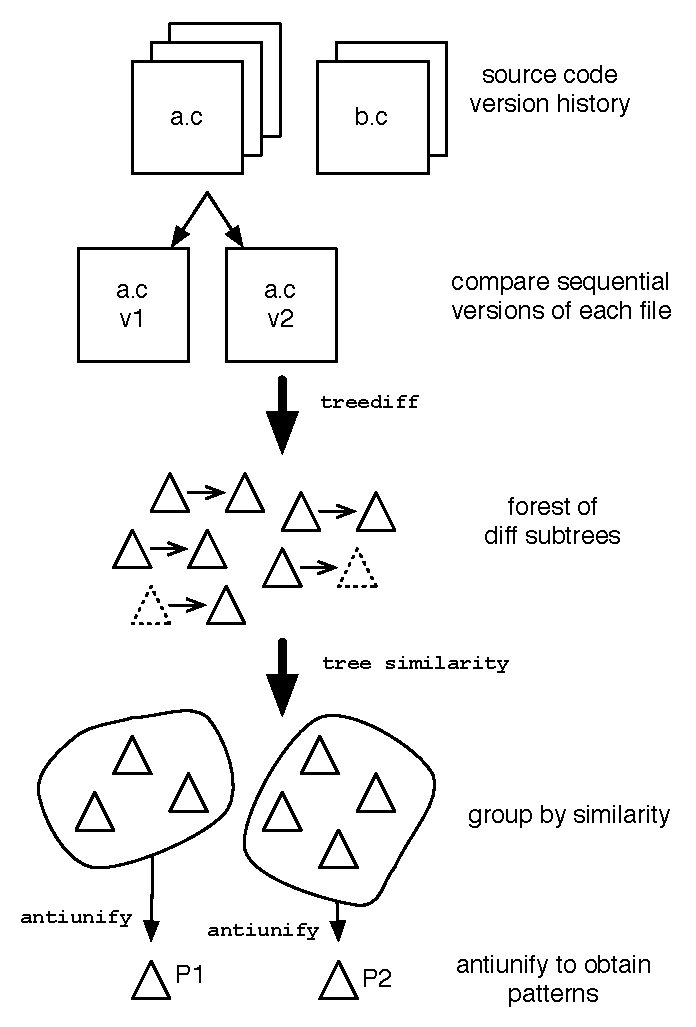
\includegraphics[height=0.44\textheight]{figures/workflow.pdf}
\caption{The components of our prototype indicating how VCS data is
broken down into groupings of related changes for pattern generation.}
\label{fig:workflow}
\end{center}
\end{figure}

Once we have code in an aterm format, we can then apply a structural
differencing algorithm between adjacent versions of each source file (e.g.,
version $n$ of file $f$ is compared to version $n+1$ of file $f$).  The result
of this is a forest of trees that represent the portions of the AST of file
$f$ that changed between versions at the structural level.  These changes can
either be code insertions, deletions, or mutations.  Our differencing is based
on the work of Yang~\cite{yang91diff} whose algorithm was designed for
computing differences between source code versions.  Yang's goal was to
improve the visual presentation of differences in textual diff tools, and our
use of their algorithm to provide input to further tree analysis algorithms is
novel.

After reducing the sequence of differences stored in the VCS, we have a large
forest of trees each representing a change that occurred over the evolution of
the software.  At this point, we seek to relate each of these trees via a
tree similarity metric.  This is achieved by using Yang's algorithm a second
time, but in this case we ignore the sequence of edit operations that it
produces and simply consume the quantitative similarity metric that it
produces as a rough estimate of how closely related two trees are.  A
threshold parameter is defined in which two trees with a similarity above the
threshold are considered to be part of the same group of difference tress.

Finally, once the set of differences are grouped into groups of trees that are
similar up to the threshold, we perform antiunification on the entire group to
distill all members to a representative code pattern for the group.
Antiunification of a set of terms yields the least general generalization of
those terms, which is how we define our notion of a code pattern.  The
antiunification algorithm as described by Bulychev~\cite{bulychev08dupe} as
part of the {\it clonedigger}
project\footnote{\url{http://clonedigger.sourceforge.net}} was used, which
itself is an implementation of the classical antiunification algorithm
described by both Reynolds~\cite{reynolds70antiunification} and
Plotkin~\cite{plotkin70antiunification}.

In the following sections, we describe the steps above in greater detail.

\subsection{Parsing and aterm generation}

One of the most challenging aspects of performing this kind of study on
arbitrary software packages is the availability of robust language parsing
tools.  In the absence of a common intermediate representation or abstract
syntax representation for popular languages, we adopted a standardized
serialization format in the form of annotated terms.  Generation of aterms was
achieved via language-specific parsers.  In this work, we used the
{\tt language-java} parser available as an open source library accessible via the
Haskell programming language.

The structure of aterms is given by this simple syntax:
\setlength{\grammarindent}{8em}
\begin{grammar}
<aterm> ::= `AAppl' <string> <aterm-list>
\alt `AList' <aterm-list>
\alt `AInt' <int>

<aterm-list> ::= <aterm> <aterm-list>
\alt $\epsilon$
\end{grammar}

This structure is sufficient for us to encode typical abstract syntax trees if
we allow ourselves to use the string label of the {\tt AAppl} portion of the
aterm. This is most easily illustrated with an example.  Suppose that we have
the Java AST for the statement {\tt i++;}.  In a textual form, this portion of
the AST would be represented by:

\begin{verbatim}
ExpStmt
  (PostIncrement
    (ExpName
      (Name [Ident "i"])))
\end{verbatim}

The translation to aterm would give us:

\begin{verbatim}
AAppl "ExpStmt"
  [AAppl "PostIncrement"
    [AAppl "ExpName"
      [AAppl "Name"
        [AList
          [AAppl "Ident" [AAppl "\"i\"" []]]]]]]
\end{verbatim}

Notice that for strings, such as identifier names, we place double quotes
around the string inside the label portion of the aterm. Implementations of
aterms often provide a representation that allows for nodes to be shared
within the tree. While this is a useful optimization for saving space, we
chose to use the simpler unshared representation in our prototype due to the
clearer expression of the tree analysis algorithms over the unshared form of
the structure.

\subsection{Structural differencing}

One of the classical algorithms studied in computer science is that of string
similarity and the concept of string edit distance as a measure of the minimal
number of operations necessary to mutate one string or sequence into another.
A more complex problem is to define a similar sequence of operations to change
a non-linear structure like a tree from one into another.  This problem of
computing a structural edit distance has been studied since the 1970s and has
yielded tree differencing algorithms analogous to string differencing
algorithms commonly used in text analysis.  Many modern efforts in this area
are based on the initial work of Selkow~\cite{selkow77tree} and
Tai~\cite{tai79tree}.  Interest in such analysis of tree-structured data
increased with the proliferation of structured document formats used on the
Internet such as XML, HTML and SGML (a noteworthy example from this body
of work is found in Chawathe~\cite{chawathe96change}).

Our work is based on Yang's source differencing technique~\cite{yang91diff}.
In this algorithm two trees to be compared are mapped to two trees of edit
operations in which nodes from the original trees are annotated with edit
operations ({\it keep} or {\it delete}).  These can be applied to turn each tree into the
other.  On their own the edit trees are not sufficient to identify the paired
subtrees that represent regions where change occurred.  This requires an
additional step of processing the edit trees to form a single tree in which the
edit trees have been woven together.

\subsection{Identifying structural changes via edit tree weaving} 
\label{sec:weaving}

Ideally, we would like to obtain from the tree differencing algorithm what can
be thought of as the two trees overlaid on each other such that the common
structure from the root towards the children is clear, and points where subtrees
differ are explicitly identified.  The details on how this algorithm was 
implemented are not critical to this paper --- instead, we will focus on what the
woven trees contain.  In the discussion that follows, we adopt the 
convention that the arguments to the binary tree differencing function are
referred to as the \emph{left} and \emph{right} trees.  

Changes that occur between the trees are represented by three change types. If
the difference between two trees is the insertion of a subtree in the right
tree, then the woven tree will contain a \emph{left-hole}.  Similarly,
deletion of a subtree from the left such that it is not present in the right
tree will result in a \emph{right-hole}.  If a subtree was determined to be
changed, then the woven tree will contain a \emph{mismatch} point that refers
to the both the right and left subtrees that differ.  All other points in the
tree that match are joined with a \emph{match} point that contains the
corresponding common node to both trees.  

Given two edit trees that have been woven together into a tree with explicit
holes and mismatches, we can extract the subtrees that correspond to the three
types of changes above.  Match points also play an important role in
extracting changes by retaining the common context that was present in both
trees where the change occurred.  If we extract only the subtree rooted at the
point where the change occurred, the rest of the analysis will be missing the
context where the change took place. This information is necessary when
constructing understandable patterns.  

For example, while it may be true that a code fragment such as {\tt i++} is
where the change occurred, it is most useful to know whether or not that
fragment occurred within an expression, a for-loop, or as a standalone
statement. As such, we have chosen for the work presented here to extract the
subtree along with the closest enclosing statement. For example, if the
subtree was the expression {\tt i++;} within the statement {\tt if(i < 100)
i++;} we would extract the if-statement with the expression.

This is achieved by including the subtree rooted at the nearest ancestor
(which must be a matching point in the woven edit trees) to a change
representing an appropriate abstract syntax element.   In the future, we would
like to explore other ways of extracting context, such as looking at the
closest enclosing expression, function (when it exists), or class.  This
information should also be parameterizable to support differences in important
AST nodes that varies between languages.

\subsection{Tree similarity metric and grouping}

Given two trees $t_1$ and $t_2$, we would like to define a similarity metric
such that $d(t_1, t_2) \in [0,1]$, where a similarity of $1$ means that the
trees are identical, and $0$ represents maximal dissimilarity.  In Yang's
algorithm, a similarity score is provided for comparing $t_a$ and $t_b$. This
metric is order dependent, forcing the maximal score to be the size of the
left tree ($t_a$), even if $t_b$ is larger.  If the trees are identical, the
score will be exactly $|t_a|$, the number of nodes in $t_a$.  If they differ,
it will be strictly less than $|t_a|$.  As such, it would be possible to define
our distance function to be $\frac{d(t_a, t_b)}{|t_a|}$, but this operator is
not symmetric, since it is easy to find instances such that $\frac{d(t_b,
t_a)}{|t_b|} \neq \frac{d(t_a, t_b)}{|t_a|}$ when the trees are very different.
Instead, we define $\Delta(t_a, t_b)$ to be the function
$$\Delta(t_a, t_b) := \frac{min(d(t_a, t_b),d(t_b, t_a))}{max(|t_a|,|t_b|)}$$
where the $min$ and $max$ functions force the calculation to be symmetric.

Once we have the set of changes that were detected from the VCS history, we
can generate a forest of trees $t_1, \cdots, t_n$ obtained from the holes and
mismatch points in the woven edit trees.  We then compute the $n^2$ distances
between all pairs to generate a distance matrix $D$ where $D_{ij} =
\Delta(t_i, t_j)$.  Given a threshold value $\tau$, we can produce a boolean
matrix $D'$ where $D'_{ij} = \Delta(t_i, t_j) > \tau$.  An example matrix is
shown in Figure~\ref{fig:boolmat} for changes observed in the VCS for ANTLR
where $\tau = 0.9$.  Note that for large numbers of changes, a sparse
representation of the boolean matrix can be computed for a given $\tau$
without requiring the full dense distance matrix to be created.  The sparsity
of the matrix is dependent both on the types of changes present and the value
of $\tau$ chosen.  

\begin{figure}
\begin{center}
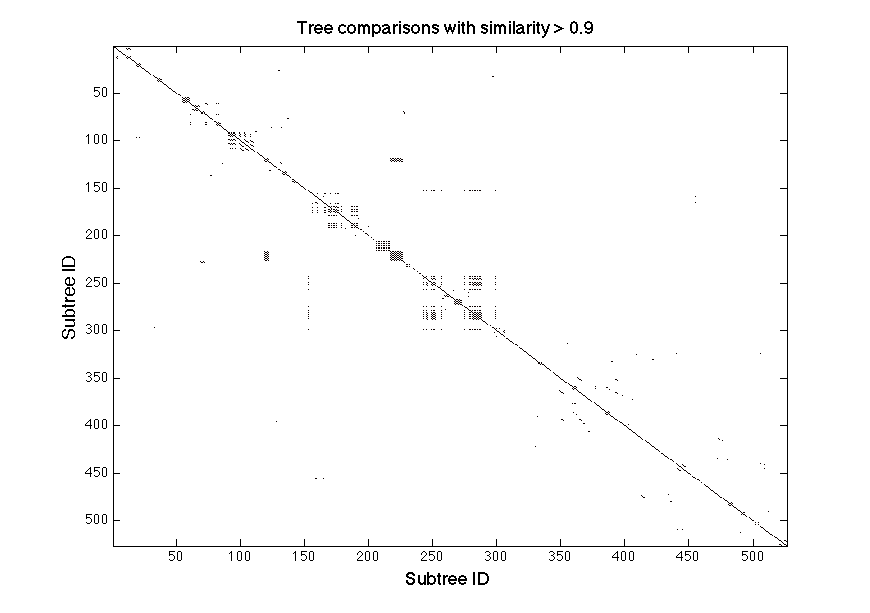
\includegraphics[width=0.45\textwidth]{figures/distmatrix-0-9.png}
\caption{Boolean matrix $D$ for over 500 changes from the ANTLR repository indicating in white all pairs of
changes for $\tau = 0.9$.}
\label{fig:boolmat}
\end{center}
\end{figure}

In our implementation, we create multiple distance matrices such that each
represents only related changes of a certain type from the woven tree (left
and right holes, and mismatches).  The matrix as defined above is simply the
element-wise boolean or of these three matrices.  Capturing this information is
important as it allows us to further refine our view of the code evolution to
distinguish code changes from the insertion or removal of code that occurs
over time. For example, when code is being developed and grown, we expect to
see a number of code insertions. Similarly, when a mass refactoring occurs to
simplify code, we would expect to see a set of code deletions.  When a more
subtle refinement occurs, such as transposition of code arguments or the
addition of a conditional to refine control flow, we would expect to see
mismatches where the tree changes.

\subsection{Antiunification and template generation}

Once we have groups of related code snippets in the form of related subtrees,
we can seek patterns that relate changes.  For example, say we have a function
call {\tt foo()} where each invocation of the function uses the same
parameters (e.g, {\tt foo(x,y)}, where {\tt x} and {\tt y} are always the
same). If we add a new parameter at the end of each call where the variable
passed in differs each time (e.g., {\tt foo(x,y,a)} and {\tt foo(x,y,b)}), we
would like to abstract out this change as {\tt foo(x,y,\metavar)}, where each
instance of the change replaces \metavar~with whatever concrete variable is
used at that point. The antiunification algorithm is built for this purpose --
given two trees, it seeks the least-general generalization of the pair and
produces a triplet representing the generalized tree with a metavariable
introduced where the two differ, as well as a substitution set that allows the
metavariable to be replaced with the appropriate concrete subtree necessary to
reconstitute the two trees that were antiunified.  Multiple distinct
metavariables (\metavar$_1$, $\cdots$, \metavar$_n$) are used when multiple
independent \metavar~points are necessary to represent a generalized set of
trees.

\section{Experimental results}

We tested the methodology outlined in section~\ref{sec:method} on the
publicly available git repositories for two popular open source
projects, the ANTLR parser generator and the Clojure language implementation.
Both are implemented in Java, and one (ANTLR) is composed of a mixture of
hand-written and automatically generated code.  

\subsection{Threshold sensitivity}

The first experiment that we performed was to investigate the effect of
similarity threshold to the number of groups identified, as well as the degree
of generality present in the tree that results from all members of each group
being anti-unified together. Our prediction was that at the lowest threshold
(0.0), when all trees are considered to be similar, their anti-unification
will yield the most general pattern.  This is what was observed, in which the
anti-unification result is a tree composed of a single metavariable node.
Similarly, at the highest threshold (1.0), the only groupings that will be
present will be single tree sets, or sets containing identical trees for
instances of identical changes that occurred in different places.  This is
precicely what we observed, with the anti-unified trees containing no meta-
variables since anti-unification of a set of identical elements is the element
itself.  We show the number of groups (broken down by type: code addition,
code deletion, or code mutation) as a function of threshold in
Figure~\ref{fig:thresholdplot}.

As we can see, as the threshold increases, we see more groupings of changes
due to changes that were considered similar under a lower threshold being
considered dissimilar under the more restrictive threshold.  For example, at
$t=0.15$, a single pattern for for-loops is identified:

\begin{verbatim}
for ([]=[];[]<[];[]) {
    []
}
\end{verbatim}

As the threshold is increased to $t=0.25$, in addition to generic for-loops, a
cohort of changes are identified to a more specific instance of the for-loop where
the loop counter is initialized to zero:

\begin{verbatim}
for ([]=0;[]<[];[]) {
    []
}
\end{verbatim}

Increasing to $t=0.35$, the pattern for the conditional becomes more specific
and we see what appears to be a template for using the field of an object
(e.g., {\tt args.length}) as the loop termination criterion:

\begin{verbatim}
for ([]=0;[]<[].[];[]) {
    []
}
\end{verbatim}

Similar templates emerge for code patterns such as method invocations, printing
the concatenation of two strings, and other common activities.  

\subsection{Group sizes}

\subsection{Pattern identification}

Using a portion of the Clojure history, we computed the number of similar trees
at each threshold. See figure~\ref{fig:clojure-number-of-modifications} to see
the number of changes by time as a function of the threshold. We looked at
thresholds from 0 to 1 with an increment size of 0.01.

\begin{figure}
\begin{center}
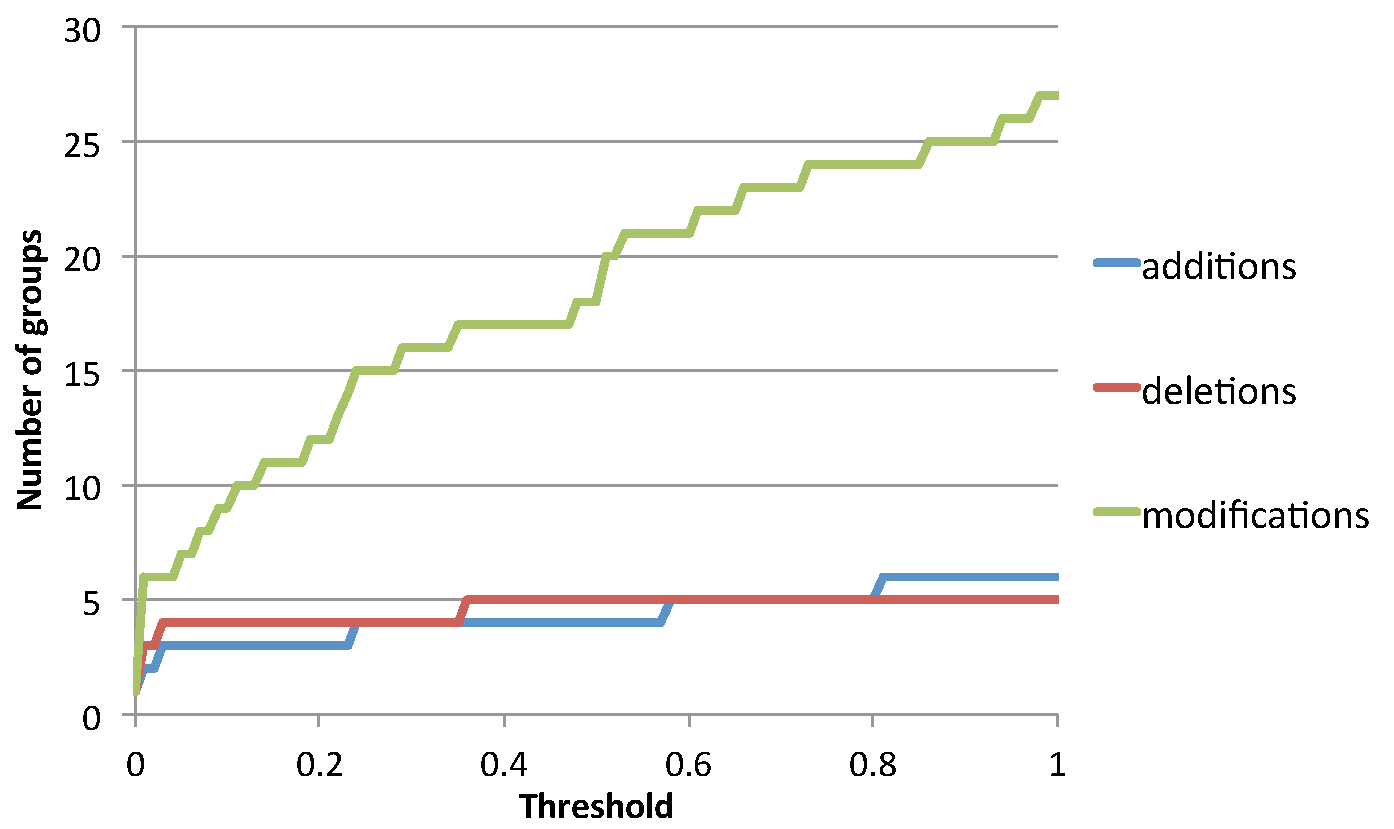
\includegraphics[width=0.44\textwidth]{figures/clojure-number-of-modifications.pdf}
\caption{Number of additions, deletions, and modifications by threshold for the Clojure source}
\label{fig:clojure-number-of-modifications}
\end{center}
\end{figure}

\begin{figure}
\begin{center}
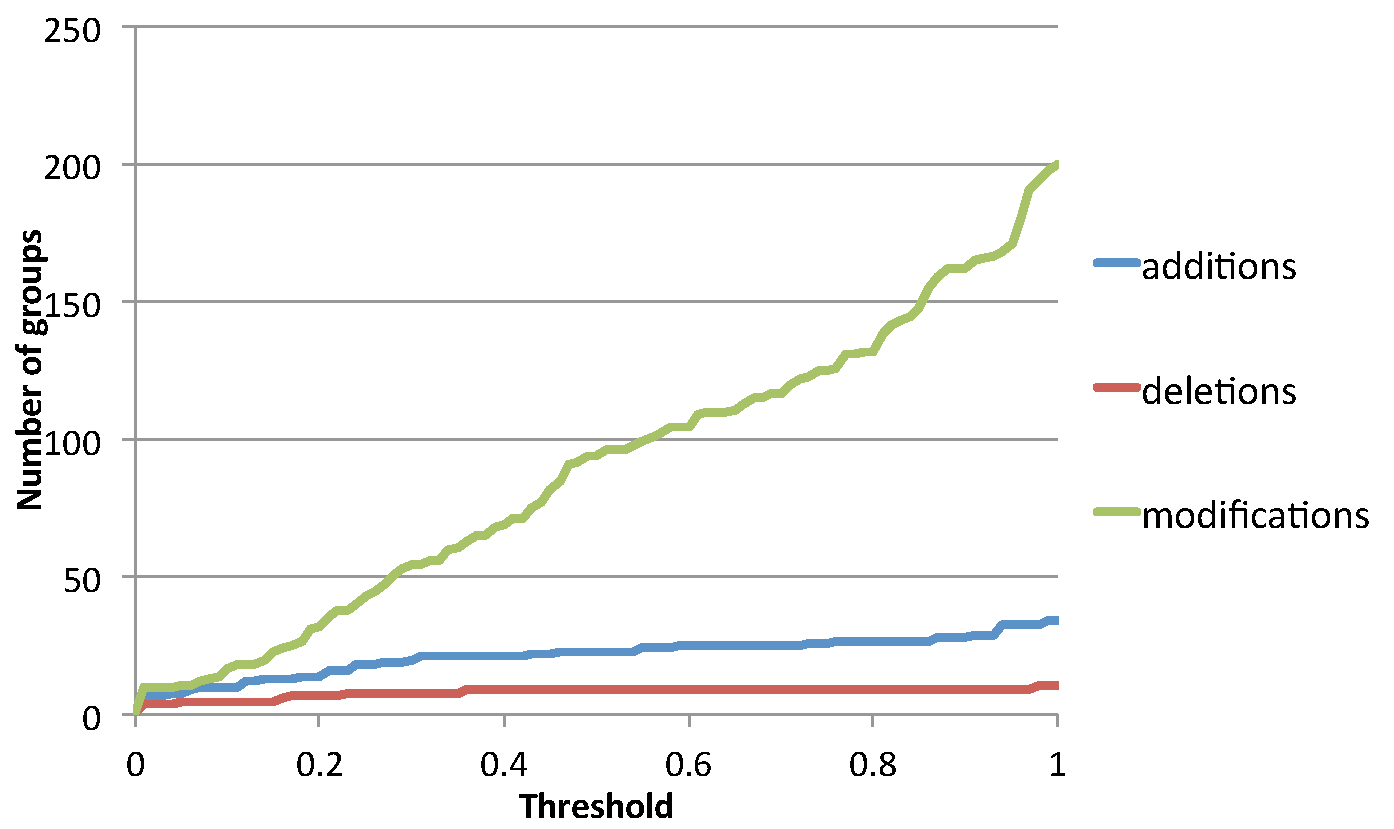
\includegraphics[width=0.44\textwidth]{figures/antlr-number-of-modifications.pdf}
\caption{Number of additions, deletions, and modifications by threshold for the Antlr source}
\label{fig:antlr-number-of-modifications}
\end{center}
\end{figure}

Looking at just the number of deletions, we examined the point where the number
of deletions goes from 4 to 5 as the threshold changes from 0.35 to 0.36.

The following code, presented in a standard diff format, shows a loop and the
lines that were removed. This example comes from a file named {\tt
PersistentArrayMap.java }.

\subsubsection{Removed code}
\begin{verbatim}
 public Object kvreduce(IFn f, Object init){
     for(int i=0;i < array.length;i+=2){
         init = f.invoke(init, array[i], array[i+1]);
-           if(RT.isReduced(init))
-                   return ((IDeref)init).deref();
         }
     return init;
 }
\end{verbatim}

Given the low threshold, this deletion was considered to be similar to the
following deletions. This example comes from {\tt PersistentHashMap.java}.
Note: Our parser ignores whitespace and gives the same AST for \verb|if (exp) { stmt; }|
and \verb|if (exp) stmt;|. In the diff below, we have prefixed the
lines that were considered to actually be different by our tool with ``>''
characters.

\begin{verbatim}
     public Object kvreduce(IFn f, Object init){
-        for(INode node : array){
-            if(node != null){
+        for(INode node : array)
+            {
+            if(node != null)
                 init = node.kvreduce(f,init);
>-                   if(RT.isReduced(init))
>-                           return ((IDeref)init).deref();
-                   }
-               }
+            }
         return init;
     }
\end{verbatim}

In both cases, our tool identified for-loops where the the same lines are
removed. In fact, the code for both of these is very similar perhaps owing to
Java's HashMap and ArrayMap classes being very similar in terms of interface.
Furthermore, it did this at the statement level, eg., we did not need to
consider the similarities of the file names or the method names.

%% Doctored version
%%\begin{verbatim}
%% public Object kvreduce(IFn f, Object init){
%%     for(INode node : array){
%%         if(node != null)
%%-        {
%%             init = node.kvreduce(f,init);
%%-            if(RT.isReduced(init))
%%-                    return ((IDeref)init).deref();
%%-        }
%%     }
%%     return init;
%% }
%%\end{verbatim}


\subsection{Interpretation of results}


\section{Conclusions and future work}

We have shown that patterns of change over the lifetime of a project can be
obtained through analysis of its version control history.  The use of tree
differencing and tree similarity measures, as well as the antiunification
algorithm for computing generalized patterns, allows this large volume of
difference data to be distilled into a compact form in which changes can be
studied at the level of the base language syntax.  Analysis of the size and
count of groups of similar changes as a function of a similarity threshold
provides a disciplined way to identify generalizations of changes identified by
the tool.

Our work has been performed using a generic, language neutral term
representation allowing the same techniques to be applied to other languages
given appropriate parsing infrastructure and a mapping from language-specific
abstract syntax forms to the generic annotated term form.  Minimal
parameterization of the tool is necessary to then consume these terms, with
language-specific parameters largely focused on specific nodes within the term
that correspond to semantically useful subtree roots for providing context to
tree differences.

In Section~\ref{sec:threshold}, we showed that our approach can highlight the
evolution of code structurally. In fact, our example of the for-loop precisely
supports the hypothetical language designer argument laid out in
Section~\ref{sec:motivation}.

In Section~\ref{sec:clojure}, we were able to find related changes in different
files that happened as part of the same commit. Not only were we able to remove
noise compared to line-based diff, but we were also looking at the Clojure
source for the first time and able to see an important relationship between the
internals of the classes in those two files. As programmers who are completely
new to the Clojure source we were able to gain valuable insight.

%% Future work after this point

Our experiment relied on a simple replay of the history of a software project.
There are other meaningful ways to generate the set of files to analyze. One
such example would be to correlate code changes to bug fixes and bug reports
and then push those changes through our workflow to find patterns.  As
mentioned in Section~\ref{sec:motivation} this may provide a support to quality
assurance practices.

In Section~\ref{sec:weaving} we explored one way to extract context. Many
different heuristics would be suitable here. Studying the trade-offs of
different heuristics would allow us to fine tune our approach depending on the
application and what we wanted to learn about the source code.

\subsection{Acknowledgments}

This work was supported in part by the US Department of
Energy Office of Science, Advanced Scientific Computing Research
contract no. DE-SC0004968.  Additional support was provided by Galois,
Inc.


%\end{document}  % This is where a 'short' article might terminate

%ACKNOWLEDGMENTS are optional

%
% The following two commands are all you need in the
% initial runs of your .tex file to
% produce the bibliography for the citations in your paper.
\bibliographystyle{abbrv}
\bibliography{sigproc}  % sigproc.bib is the name of the Bibliography in this case
% You must have a proper ".bib" file
%  and remember to run:
% latex bibtex latex latex
% to resolve all references
%
% ACM needs 'a single self-contained file'!
%
%% %APPENDICES are optional
%% %\balancecolumns
%% \appendix
%% %Appendix A
%% \section{Headings in Appendices}
%% The rules about hierarchical headings discussed above for
%% the body of the article are different in the appendices.
%% In the \textbf{appendix} environment, the command
%% \textbf{section} is used to
%% indicate the start of each Appendix, with alphabetic order
%% designation (i.e. the first is A, the second B, etc.) and
%% a title (if you include one).  So, if you need
%% hierarchical structure
%% \textit{within} an Appendix, start with \textbf{subsection} as the
%% highest level. Here is an outline of the body of this
%% document in Appendix-appropriate form:
%% \subsection{Introduction}
%% \subsection{The Body of the Paper}
%% \subsubsection{Type Changes and  Special Characters}
%% \subsubsection{Math Equations}
%% \paragraph{Inline (In-text) Equations}
%% \paragraph{Display Equations}
%% \subsubsection{Citations}
%% \subsubsection{Tables}
%% \subsubsection{Figures}
%% \subsubsection{Theorem-like Constructs}
%% \subsubsection*{A Caveat for the \TeX\ Expert}
%% \subsection{Conclusions}
%% \subsection{Acknowledgments}
%% \subsection{Additional Authors}
%% This section is inserted by \LaTeX; you do not insert it.
%% You just add the names and information in the
%% \texttt{{\char'134}additionalauthors} command at the start
%% of the document.
%% \subsection{References}
%% Generated by bibtex from your ~.bib file.  Run latex,
%% then bibtex, then latex twice (to resolve references)
%% to create the ~.bbl file.  Insert that ~.bbl file into
%% the .tex source file and comment out
%% the command \texttt{{\char'134}thebibliography}.
%% % This next section command marks the start of
%% % Appendix B, and does not continue the present hierarchy
%% \section{More Help for the Hardy}
%% The acm\_proc\_article-sp document class file itself is chock-full of succinct
%% and helpful comments.  If you consider yourself a moderately
%% experienced to expert user of \LaTeX, you may find reading
%% it useful but please remember not to change it.
%% \balancecolumns
%% % That's all folks!
\end{document}
